\begin{refsection}
In this chapter, the methodology followed for the development of this thesis will be carried out. This section is going to be divided into two main parts. The first one will describe the experimental procedures carried out, including the linseed oil oxidation kinetic determination, the silica micro-capsules synthesis, the OS film elaboration, and the head-space oxygen concentration evolution test. The second part will refer to the computational procedure followed for the development of the design tool program; this includes the physical model description, the numerical resolution approach, the kinetic parameters adjustment strategy, and finally, the graphical user interface (GUI) programming. 

\section[Exp.Procedure]{Experimental Procedure}
\subsection{Materials}\label{subsec:materials}
Before describing the procedure followed to synthesize active silica microcapsules containing linseed oil and describing the active film elaboration methodology, it is essential to state the materials used in these experimental procedures. The materials used are listed in the table \ref{tab:material}

\begin{table}[h]
\centering
\caption{Materials used in the experimental procedure for the synthesis of 2g of micro-capsules and for a 17cmx17cm polymeric film.}
\label{tab:material}
\begin{tabular}{|c|c|}
\hline
Material                        & Quantity (per batch) \\ \hline
Ethanol  Absolute               & 36 mL                \\ \hline
Deionized  Water                & 85.5 mL              \\ \hline
Cetrimonium  Bromide (CTAB)     & 0.48 g               \\ \hline
Linseed  Oil                    & 1.5 mL               \\ \hline
Tetraethylorthosilicate  (TEOS) & 6 mL                 \\ \hline
25\% Ammonia Solution           & 3 mL                 \\ \hline
High Density Polyethylene (HDPE) Homopolymer & 62 g            \\ \hline
\end{tabular}
\end{table}

Double cooked linseed oil was supplied by \textit{Produquímica de Colombia S.A.} The composition of the oil is shown in Table \ref{tab:oil_composition}. For the headspace oxygen analysis, 8cm by 18cm triple-layer bags (with layers of polypropylene, metallic polyester, and low-density polyethylene) were used.

\begin{table}[h]
 \centering
 \caption{Double cooked linseed oil composition obtained by gas chromatography}
  \begin{tabular}[htbp]{@{}ll@{}}
    \hline
    Name & Composition \% wt\\
    \hline
    Palmitic Acid  & 4-8 \\
    Stearic Acid   & 2-6 \\
    Oleic Acid & 16-23\\
    Linoleic Acid & 13-18 \\
    Linolenic Acid & 50-60 \\
    Other fatty Acid & Max 1\\
    \hline
  \end{tabular}
  \label{tab:oil_composition}
\end{table}

\subsection{Silica micro-capsules synthesis}\label{subsec:met.sintesis}
Regarding the microcapsule synthesis, this has been carried out by the CIPP-CIPEM using the sol-gel emulsion templating methodology. This procedure consists of preparing an emulsion in which the dispersed phase is the chemical species that is desired to be encapsulated. In this case, the surfactant or emulsifier will serve as a template where the tetraethyl orthosilicate (TEOS) precursor undergoes hydrolysis and condensation reactions to form the silica polymeric microcapsule \cites{Alvarado2020ValidacionesEncapsulados}. To obtain 2.34g of dry product, initially, 85.5 mL of water, 0.48g of cetrimonium bromide (CTAB), and 36mL of ethanol are mixed in a 250mL beaker with a rotational speed of 700rpm for 5 minutes. Afterward, 1.5 mL of double-cooked linseed oil is added drop by drop to the previous mix, and immediately after, 6mL of TEOS is slowly added to the beaker, which is left mixing for 5 minutes. Finally, 3mL of 25\% ammonia solution is added to the beaker to catalyze the reaction, which is left mixing at 700 rpm for 24 hours. The mix obtained is centrifuged at a velocity of 4000 rpm for ten minutes; thus, the micro-capsules obtained are separated from the liquid phase of the mix. Next, the solid were dried in a vacuum oven at 70\degree C and a pressure of $-0.06 MPa$ for 4 hours. After that time, the microcapsules are ready to be incorporated into the polymeric film. In the figure\ref{fig:capsules}, an image of the product obtained is shown. 


\begin{figure}[h]
    \centering
    \begin{subfigure}[b]{0.3\linewidth}           \centering
        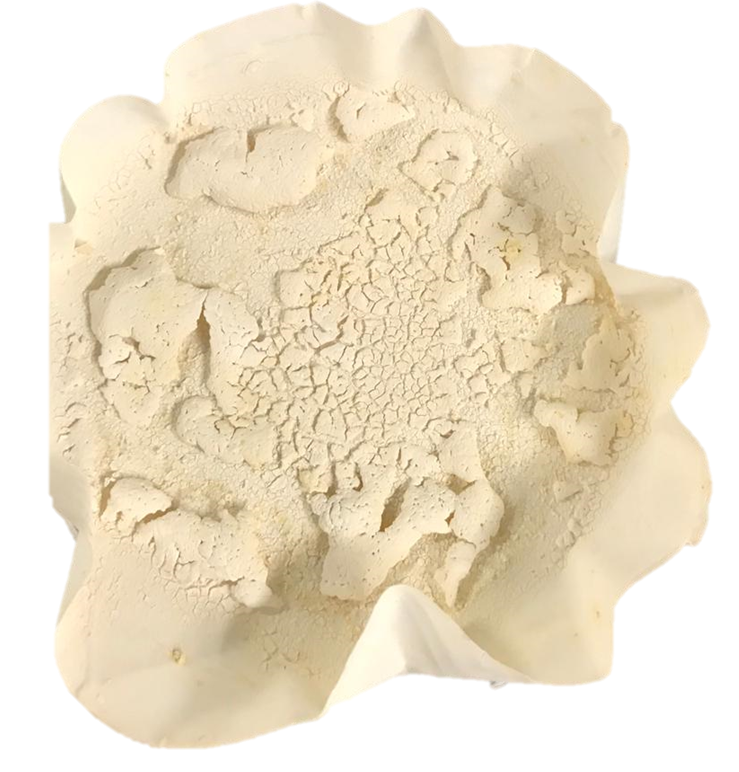
\includegraphics[width=\linewidth]{Documento_Latex/Tesis_2/Imagenes/capsulas (2).png}
    \end{subfigure}
    \begin{subfigure}[b]{0.3\linewidth}
        \centering
        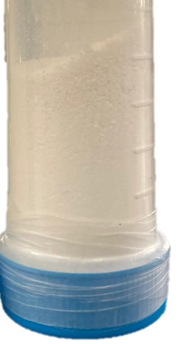
\includegraphics[width=0.5\linewidth]{Documento_Latex/Tesis_2/Imagenes/capsulas.png}
    \end{subfigure}
    \caption{Silica microcapsules obtained by the methodology described in section \ref{subsec:met.sintesis}}
    \label{fig:capsules}
\end{figure}

\subsection{Film Elaboration} \label{sec:film_elaboration}
The film elaboration refers to the different processes between incorporating the silica micro-capsules into the polymeric film's final production. Regarding incorporating the capsules, once having 9g of this, a masterbatch (MB) is prepared by mixing the microcapsule load and high-density polyethylene (HDPE) homopolymer within an internal mixer which has to be preheated 10 minutes before at 170\degree C. The ratio of micro-capsules to HDPE in the mix was 20:80 mass proportion, respectively. This mix is poured into the internal mixer for 7 minutes, during which the torque and temperature are monitored until these two signals stabilized, indicating a homogeneous mixture. The material obtained must be frozen to a temperature of -80\degree C for 3 hours in an ultra-freezer. This process is necessary to increase the fragility of the material. Afterward, it was taken into a blade mill for grinding for 1 minute, and in this way, the masterbatch (MB) was finished. \\

Next, the masterbatch previously obtained was diluted with HPDE homopolymer to form the films; a mix of 10g of MB and 30g of HPDE was submitted through the same mixing process as the Masterbatch did. Finally, the process of compression molding is done by using a press;  two aluminum foils and two Teflon foils are put over the two sides of the press, and in the inferior part of it, a quantity of 12g of the HDPE-MB mixture is poured into a 17cm x 17cm aluminum frame with a 3cm width. The inferior and superior plates are both preheated to a temperature of 170\degree C, and the press must be configured so that an initial pressure of 15 bar is applied for 1 minute, and then a pressure of 110 bar must be applied for 1.5 minutes, after which a 10 minutes cooling time is done. After this, the desired film of 17cm x 17cm with OS load is obtained (Figure \ref{fig:film}).

\begin{figure}[ht]
    \centering
    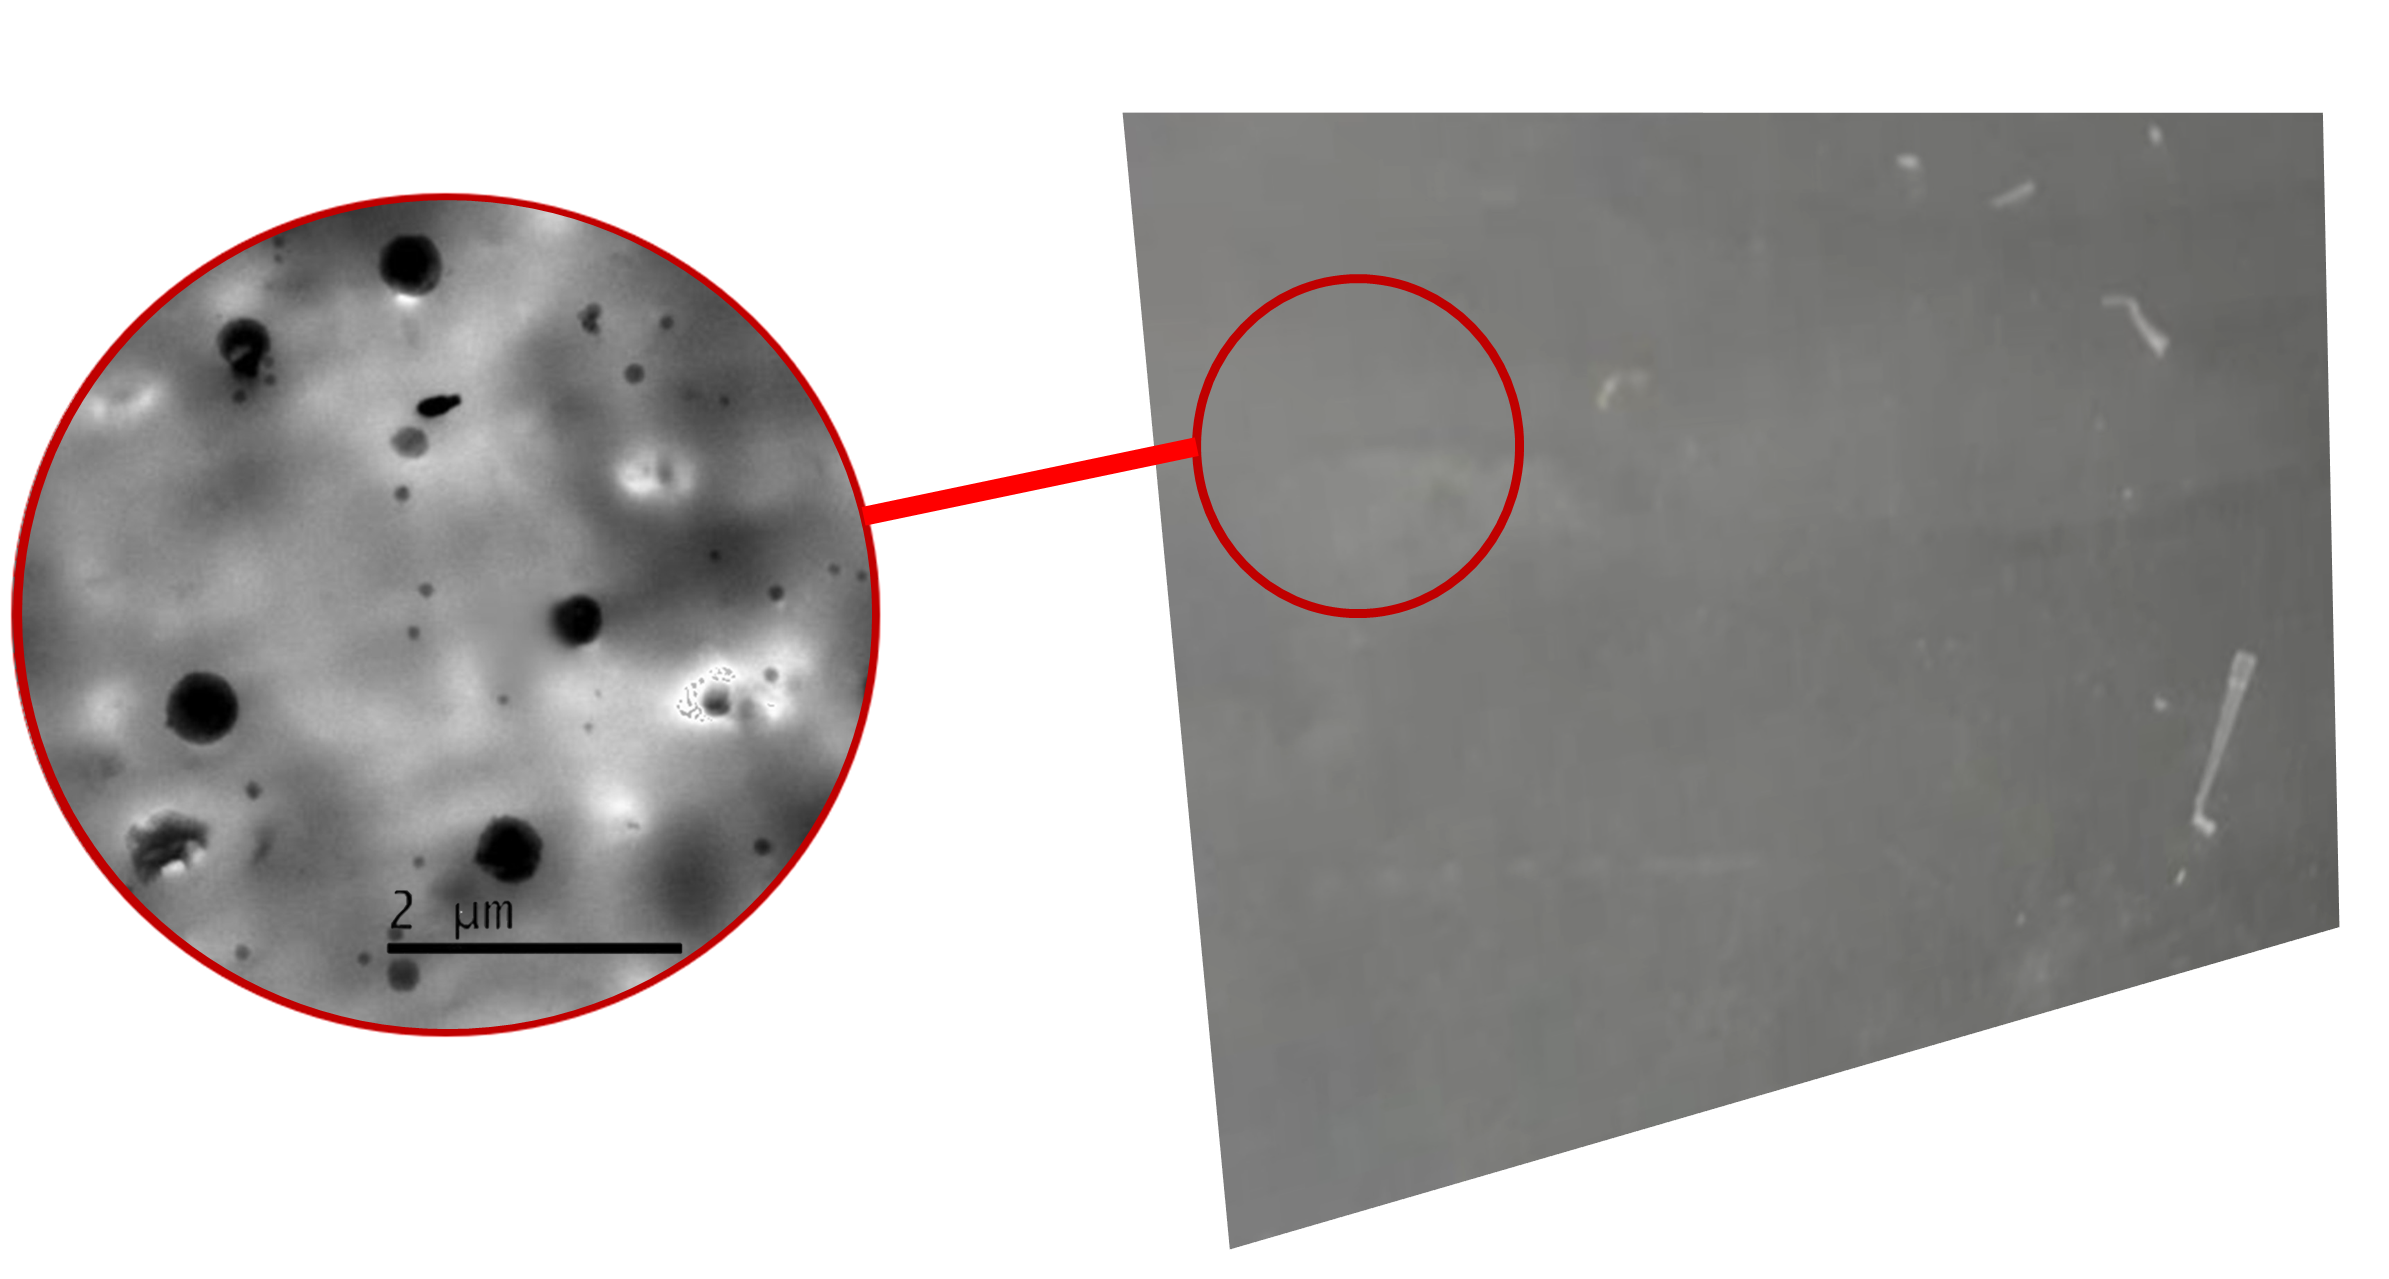
\includegraphics[width=0.6\linewidth]{Imagenes/pelicula.png}
    \caption{HPDE film containing silica microcapsules which were incorporated following the methodology described in section \ref{sec:film_elaboration} \cite{ArellanoAyala2019EfectosAntioxidantes}}
    \label{fig:film}
\end{figure}

\subsection{Headspace Oxygen Absorption Test}\label{sec:headspace}
The headspace is defined in the packaging industry as the volume of gas inside a package. In this case, the evolution of the oxygen concentration within the head-space gas of a control volume was used as the main experiment to verify the physical model's prediction capacity and numerical solutions throughout this thesis.  This test was done using a Quantek 901 head-space oxygen analyzer. This equipment can measure oxygen concentrations going from 0.1\% v/v to 100\%v/v with a 0.1\% v/v precision. The operating principle of the Quantek 901 is based on a fuel cell oxygen sensor, which consists of a diffusion barrier, a sensing electrode made of platinum, and a working electrode made of zinc, all submerged in a solution of potassium hydroxide, which acts as an electrolyte \cite{Boissevain1996CorporateGuide}. The entering oxygen diffuses into the sensor and reduces to hydroxyl ions at the cathode, as shown in reaction \ref{reacc:head_spc_1} \reaction[reacc:head_spc_1]{O2 +2H2O +4e^- -> 4OH^-\text{.}} Next, the hydroxyl ions formed are oxidized at the zinc anode (reaction \ref{reacc:head_spc_2}) .
 \reaction[reacc:head_spc_2]{2Pb + 4OH^- -> 2PbO +2H2O + 4e^-\text{,}}
 which yields an overall cell reaction as the one shown in reaction \ref{reacc:head_spc_3}.
 \reaction[reacc:head_spc_3]{2Pb + O2 -> 2PbO}

 
 The current generated during this reaction is proportional to the concentration of oxygen present in the medium. With this in mind,  the sensor measures these currents and calculates the amount of oxygen within a gas sample \cite{GarciaMora2015KineticScavengers, Boissevain1996CorporateGuide}.\\
 
 The headspace oxygen analysis was carried out for silica micro-capsules and 5\% OS HPDE films. Several 8cm by 18cm triple-layer bags (see figure \ref{fig:non_sealed_bag}) were used to carry out this test. To test the nanomaterial, 0.6g of it was introduced into the bag, while for testing the films, a sample of 8cm by 14cm was added to the bag. Once the samples which were going to be tested were within the bags, these were sealed using a Sentinel Heat Sealer 12AS from Packaging Industries Inc., as shown in the figure\ref{fig:sealer}. This equipment was preheated to a temperature of 400\degree C, and the bags were pressed within the sealer for 4 seconds, after which the bag was sealed as shown in the figure \ref{fig:sealed_bag}.  
 
 \begin{figure}[htbp]
    \centering
    \begin{subfigure}[b]{0.3\linewidth}           \centering
        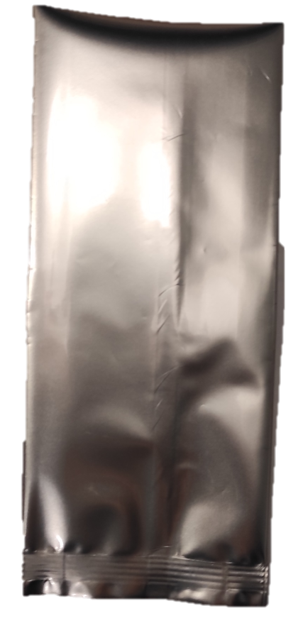
\includegraphics[width=0.5\linewidth]{Documento_Latex/Tesis_2/Imagenes/Non_Sealed_Bag.png}
        \caption{ }
        \label{fig:non_sealed_bag}
    \end{subfigure}
    \begin{subfigure}[b]{0.3\linewidth}
        \centering
        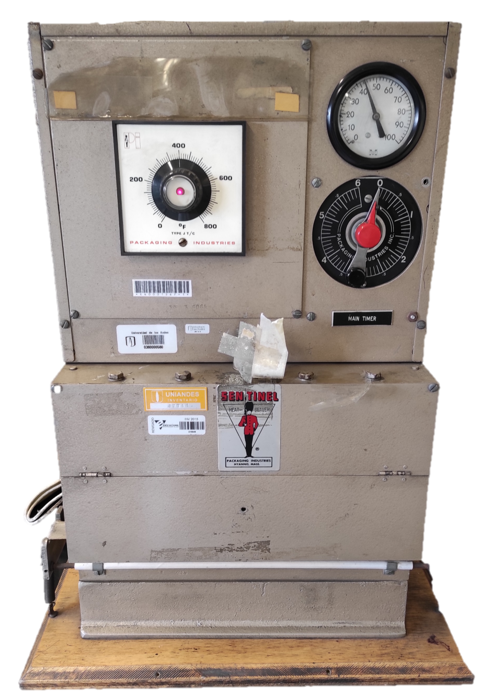
\includegraphics[width=0.8\linewidth]{Documento_Latex/Tesis_2/Imagenes/Sealer.png}
        \caption{ }
        \label{fig:sealer}
    \end{subfigure}
    \begin{subfigure}[b]{0.3\linewidth}
        \centering
        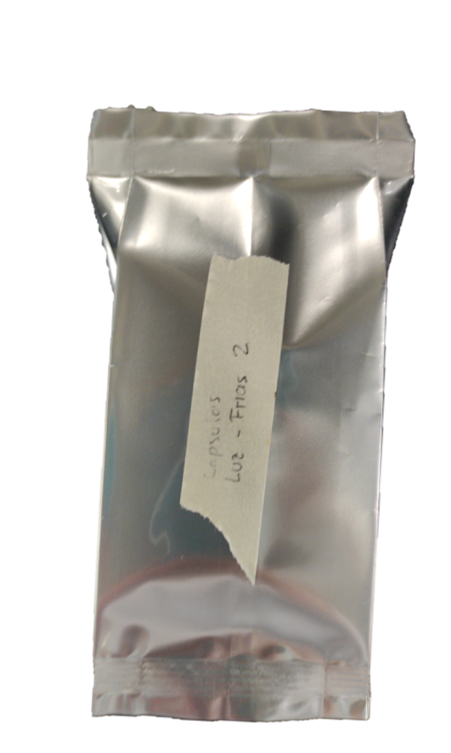
\includegraphics[width=0.8\linewidth]{Documento_Latex/Tesis_2/Imagenes/Sealed_Bag.png}
        \caption{ }
        \label{fig:sealed_bag}
    \end{subfigure}
    \caption{Representation of the bags used for the headspace experiment \textbf{a)} before sealed and \textbf{c)} after sealed,  by using the heat sealer shown in image \textbf{b)}}
    \label{fig:bags}
\end{figure}

Once the bags were sealed, they were filled with 120mL of air; this was done by sticking an adhesive acrylic with a polyethylene liner septa to the bag's surface and injecting through it the desired quantity of air with a graduated syringe. The septa are used to prevent that air gets into the bag once they are stabbed, so the headspace atmosphere is only altered by the presence of capsules or the film within it.

Moreover, it is essential to clarify that the tests for the 1.2g of capsules and the 5\% OS HPDE films were made in triplicate and that a negative control was set by filling three bags with only air to monitor that the oxygen concentration within them remains stable throughout the test. \\

Finally, to carry out the headspace oxygen concentration test, a bag must be punctured through the EPDM septa using the needle attached to the Quantek Oxygen Analyser. This equipment was calibrated to take a sample of 2mL of headspace gas within the test bag, this is analyzed by the equipment, which finally reports the volumetric oxygen concentration in the headspace gas (See figure \ref{fig:headspace_test_image}). The tests made were destructive, meaning that once a bag was punctured to do a measurement, it was immediately discarded. This approach assumes that the oxygen absorption behavior in each bag will be equal in all the bags and has the advantage (over the nondestructive approach) that it does not allow the leakage of atmospheric oxygen due to successive measurements over the same bag. 


Each measurement was made every 48 hours, and a total of 6 data points were taken (which cover up a total time of 340 hours).

\begin{figure}[h]
    \centering
    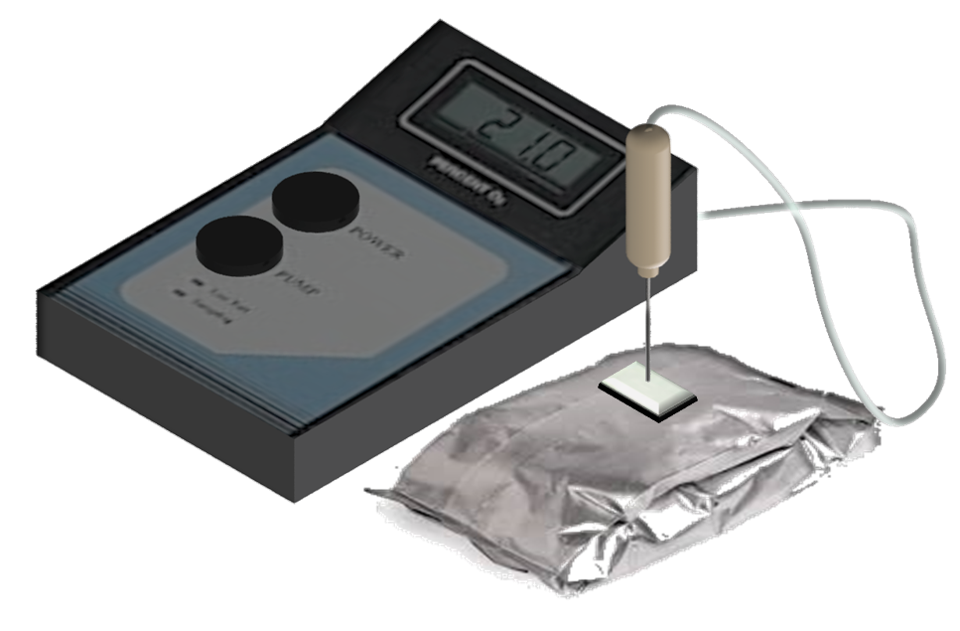
\includegraphics[width=0.7\textwidth]{Documento_Latex/Tesis_2/Imagenes/Headspace_test.png}
    \caption{Representation of the oxygen headspace concentration test assembly.}
    \label{fig:headspace_test_image}
\end{figure}
 
\subsection[Oxidative TGA]{Oxidative Thermogravimetric Analysis}\label{sec:TGA} 
It is crucial to determine the oxidation kinetics of double-cooked linseed oil to carry on the development of the design tool. Given that in the autoxidation
process described in Section \textbf{X}, there is an increase in the weight of oils due to the absorption of oxygen from the environment. Even though these weight changes are minimal, they are big enough for being detected in the thermogravimetric analysis (TGA). The TGA test in several atmospheres and temperatures was carried over double-cooked linseed oil samples to establish the oil autoxidation reaction constants.\\


All tests were made using a simultaneous TGA-DSC SDT Q600 (TA instruments) with a sample of 26mg of linseed oil and at a heating rate of 20\degree C. The different conditions used in every TGA run made are shown in the table \ref{tab:TGA_test}

\begin{table}[h]
\centering
\caption{Linseed oil TGA test conditions evaluated to determine the oxidation kinetics constants.}
\label{tab:TGA_test}
\begin{tabular}{|c|c|c|}
\hline
Sample &
  Atmosphere &
  Temperature {[}\degree C{]} \\ \hline
\multirow{9}{*}{\begin{tabular}[c]{@{}c@{}}Linseed Oil\\  (26mg)\end{tabular}} &
  \multirow{3}{*}{Nitrogen UAP} &
  25 \\ \cline{3-3} 
 &                          & 40 \\ \cline{3-3} 
 &                          & 80 \\ \cline{2-3} 
 &
  \multirow{3}{*}{\begin{tabular}[c]{@{}c@{}}Oxygen UAP 70\% v/v - \\ Nitrogen UAP 30\% v/v\end{tabular}} &
  25 \\ \cline{3-3} 
 &                          & 40 \\ \cline{3-3} 
 &                          & 80 \\ \cline{2-3} 
 & \multirow{3}{*}{Dry Air} & 25 \\ \cline{3-3} 
 &                          & 40 \\ \cline{3-3} 
 &                          & 80 \\ \hline
\multicolumn{2}{|c|}{Time per test run {[}h{]}} &
  24 \\ \hline
\end{tabular}
\end{table}

 The first TGA test carried out was under a nitrogen atmosphere; this were done to observe the sole effect of airflow around linseed oil and OS films. In this case, the volatile components within the sample will evaporate, generating a reduction in the measured mass. The second TGA test made used a pure oxygen atmosphere as the purge gas; in this case,  oxygen is in excess concerning the substrate, so the kinetics of oxidation can be simplified, as explained in Section 1.2.4. 
The change in the mass of the sample obtained is normalized by the mass reduction due to the evaporation obtained from the nitrogen atmosphere TGA. In this way, there is a guarantee that the mass changes of the oxygen TGA are exclusively due to oxygen absorption. The third and final TGA made was in an air atmosphere, in which oxygen has a concentration of 20.6 vol\%. Contrary to the case of oxygen atmosphere TGA, in this case, it is not correct to assume that oxygen is in excess, so the results obtained in this test must be compared to the complete autoxidation kinetics of the linseed oil.
 
\section[Comp.Procedure]{Computational Procedure}
The mathematical models used are explained in this section to understand the limitations of the design tool. It is essential to comprehend how linseed oil oxidation kinetic was determined given that this enables to understand and fully model linseed oil; this was done by proposing a closed-loop oxidative mechanism of 6 reactions that predicts linseed oil's mass gain profile during an oxidative TGA. Once the reacting behavior of linseed oil is modeled, it was included in the mathematical models which described the active film oxygen absorption. When modeling this system, two approaches were considered, the reactive film (homogeneous) approach and the heterogeneous (active site) approach; each of these is explained in sections \textbf{X} and \textbf{Y}, respectively. Given the simplicity of the reactive film model, it was expanded to consider a multilayer material in which one or multiple layers can have nanocapsules which make the respective layers reactive, this is explained in section \textbf{Z}. Finally,  several numerical methods were evaluated to solve the mathematical models previously mentioned to find which one was able to obtain a concentration profile with a minor error and in less computational time, this is explained in section \textbf{A}. 


\subsection{Kinetic parameters adjustment}\label{subsec:met_cinetica}
Linseed oil oxidation has been widely studied due to its applicability in drying paints. As stated in the literature review section, few studies aim to determine the value of kinetic parameters of linseed oil oxidation at low temperatures. Based on the closed-loop oxidation mechanism proposed for hydrocarbon oxidation which has been used to describe substrate oxidation with only one type of reactive site, the following reactive scheme is proposed to describe linseed oil reaction with oxygen.

\begin{subequations}
\begin{gather}
    Initiation:\nonumber\\
    ROOH+ROOH \xrightarrow{k_1}ROO^\cdot+\text{carbonyl}+R^\cdot +\text{Scission}\\
    Propagation:\nonumber\\
    R^\cdot+O_2 \xrightarrow{k_2}ROO^\cdot \label{eq:propagation_oxygen}\\
    ROO^\cdot+ RH\xrightarrow{k_3}ROOH+R^\cdot \label{eq:propagation_substrate}\\
    Termination:\nonumber\\
    R^\cdot+R^\cdot \xrightarrow{k_4}\text{inactive product}\\
    R^\cdot+ROO^\cdot\xrightarrow{k_5}\text{inactive product}\\
    ROO^\cdot+ROO^\cdot\xrightarrow{k_6}\text{inactive product}
\end{gather}
\label{eq:reacciones_cinetica}
\end{subequations}

This reaction mechanism consists of three stages, the first one being an initiation stage where bimolecular decomposition of hydroperoxides ($ROOH$) generates alkyl and peroxyl radicals ($R^\cdot$, $ROO^\cdot$). In this case, the mechanism did not consider the unimolecular decomposition of hydroperoxides, given that the experimental activation energy for the induction period is approximately 110kJ/mol. In contrast, the activation energy for unimolecular decomposition is higher than 140 kJ/mol, suggesting that this mechanism is not likely to occur \cite{Richaud2012RateChemiluminescence,Denisov2005OxidationBiology}. The second stage is the propagation step in which oxygen ($O_2$) and the substrate ($RH$) react with the radicals produced in the initiation step. In this case, the substrate is the double bond in $\alpha$ position in the fatty acids
that compose the oil (mainly oleic, linoleic, and linolenic). The propagation step is where the close loop mechanism occurs. The reaction \ref{eq:propagation_oxygen} consumes oxygen and alkyl radicals but generates  additional peroxyl radicals, which reacts with the substrate in the oil (reaction \ref{eq:propagation_substrate}) and produces hydroperoxides which are the reactive species in the initiation reaction  generating a reactive loop. The third and final stage of the reaction mechanism is the termination reactions in which radical species react to produce inactive products. \\ 

Based on the reactive mechanism proposed for linseed oil oxidation, the kinetic scheme in equation \ref{eq:equaciones_cinetica}is formulated. 

\begin{subequations}
\begin{gather}
    \frac{d[ROOH]}{dt}=-2k_1[ROOH]^2+k_3[ROO^\cdot][RH]\\
    \frac{d[RH]}{dt}=-k_3[ROO^\cdot][RH]\\
    \frac{d[ROO^\cdot]}{dt}=k_1[ROOH]^2+k_2[R^\cdot][O_2]-k_3[ROO^\cdot][RH]-k_5[ROO^\cdot][R^\cdot]-2k_6[ROO^\cdot]^2\\
    \frac{d[R^\cdot]}{dt}=k_1[ROOH]^2-k_2[R^\cdot][O_2]+k_3[ROO^\cdot][RH]-2k_4[R^\cdot]^2-k_5[ROO^\cdot][R^\cdot]\\
    \frac{d[O_2]}{dt}=-k_2[R^\cdot][O_2]
\end{gather}
\label{eq:equaciones_cinetica}
\end{subequations}

The solution of the previous equations through numerical methods enables the prediction of the concentration profiles of the different reactive species in reactions \ref{eq:reacciones_cinetica}. To solve the system of ODE,  the reaction velocity constants ($k_1$ to $k_6$), as well as the initial concentration of the reactive species, have to be known. These values are determined by adjusting the mass oil gain in oxidative TGA at different temperatures. As shown in reaction \ref{eq:propagation_oxygen}, the alkyl radicals present in the oil react with oxygen to produce peroxyl radicals; this reaction traduces to an increment in the oil mass, which the TGA detects during an oxidative test. With this in mind, it is possible to relate the oxygen consumption rate with linseed oil's mass gain through equation \ref{eq:mass_gain} . 

\begin{equation}
    \frac{dm}{dt}=\frac{M_{O_{2}}}{\rho_{oil}}k_2[R^\cdot][O_2]
    \label{eq:mass_gain}
\end{equation}

In equation \ref{eq:mass_gain},  $M_{O_{2}}$ represents the molecular weight of oxygen, $\rho_{oil}$ the density of linseed oil, $k_2$ the rate constant of equation,\ref{eq:propagation_oxygen} and $[R]$ and $[O_2]$ represents the concentration of alkyl radical and oxygen in the oil (in mol/m3). Employing numerical methods equation \ref{eq:mass_gain} can be solved to predict a mass profile for linseed oil as a function of time.  The profile obtained was compared to the experimental TGA mass profile for linseed oil by calculating the sum of squares of the residuals of the predicted profile. The sum of the errors was used as an objective function which was minimized by changing the initial concentration values of the species and the kinetics constants in equation \ref{eq:equaciones_cinetica} (See equation \ref{eq:funcion_objetivo}). 

\begin{equation}
    min \sum_{i=0}^n\left(m(t_i,k)-\hat{m}_i\right)^2
    \label{eq:funcion_objetivo}
\end{equation}

The minimization was done using the Levenberg–Marquardt algorithm; the initial condition to solve equation \ref{eq:equaciones_cinetica}considered that the oil has a concentration of hydroperoxides and substrate $[ROOH]_o$, $[RH]_o$, while having a constant concentration of oxygen $[O_2]=S_{O_2}P_{O_2}$. On the other hand, radicals are going to be considered to have an initial concentration of zero. As initialization value for the adjustment of $[ROOH]_o$, $[RH]_o$, the concentration values determined by Richaud et al. \cite{Richaud2012RateChemiluminescence} for methyl linolenate were used given that linseed oil is composed mainly of linolenic acid (see Table \ref{tab:oil_composition}).


\subsection{Reactive Film Model }\label{subsec:reactive_film_met}
The first model developed to predict the performance of oxygen uptake from the OS films made, is the reactive film model. This approach assumes that the nanocapsules containing linseed oil are sufficiently and homogeneously dispersed in the polymeric matrix so that the system can be model as if the film was a reactive media and the oxygen reacts through the whole film volume, not only in specific active sites. By using this approach, the OS film system is simplified allowing quick prediction of the oxygen uptake profiles.

To establish this model, consider a film of Area $A$ and thickness $L$, which is inside a control $V$ and at constant temperature $T$. The gas in the bottle considered has an initial oxygen molar concentration $C_{ext_o}$. The situation described is shown in figure \ref{fig:model_diagram}. 



 
  \end{refsection}